\documentclass[10pt,a4paper]{article}
\usepackage[latin1]{inputenc}
\usepackage{amsmath}
\usepackage{amsfonts}
\usepackage{amssymb}
\usepackage{graphicx}
\usepackage{geometry}
\usepackage{tikz}
\usepackage{todonotes}
\usepackage{amsthm}
\usepackage{tabularx}
    \newcolumntype{L}{>{\raggedright\arraybackslash}X}

\geometry{a4paper, top=25mm, left=40mm, right=25mm, bottom=30mm,
	headsep=10mm, footskip=12mm}
\title{Statistisches Lernen\\ \large{Vorlesung Wintersemester 17/18}\\
}

\def\firstcircle{(0,0) circle (1.5cm)}
\def\secondcircle{(45:2cm) circle (1.5cm)}
\def\thirdcircle{(0:2cm) circle (1.5cm)}
\date{} 

\theoremstyle{definition}
\newtheorem{exmp}{Beispiel}
\newtheorem{axiom}{Axiom}
\begin{document}
	\maketitle
	
	\begin{center}
		https://www.imise.uni-leipzig.de/Lehre/Semester/2017-18/BI-Bioinformatik/index.jsp\\
		Bemerkung 1: dienstags, HS13, donnerstags HS19\\
		Bemerkung 2: Login Name: StudentSL, Pwd: DateienSL
	\end{center}

%Vorlesung 1
	\section{Einführung}
	\subsection{Vorbemerkungen}
	\begin{itemize}
		\item Bei statistischem Lernen geht es darum intelligente Schlüsse aus Daten zu ziehen
		\begin{itemize}
			\item Fokus auf Methoden zu Analysen
			\item wenig/nicht über Design
			\item viele Bsp. aus dem Bereich der klinischen Studien
			\item Anwendungen auf ganz anderen Gebieten
		\end{itemize}
	\item Beispielhafte Anwendungen
	\begin{itemize}
		\item Unterscheiden sich Behandlungen A und B
		\item Was sind die Eigenschaften eines diagnostischen Test
		\item Gibt es einen Zusammenhang zwischen Krankheiten A und B
	\end{itemize}
	\end{itemize}
\subsection{Wahrscheinlichkeit}
\subsubsection{Zugänge}
\begin{itemize}
	\item relative Häufigkeit (frequentistisch)
	\item Maß für eine Überzeugung (Bayes'sche Statistik)
\end{itemize}
\textbf{frequentistisch:} intuitiv, basiert auf wiederholbaren ''Experimenten'' (z.B. Münzwurf, radioaktiver Zerfall, Schwangerschaft bei Kontrazeptionsmethode(Verhütungsmethode) A, 5-Jahre Überleben nach Chemotherapie, Regen am nächsten Tag in Leipzig)

\begin{itemize}
	\item in den ersten Vorlesungen folgen wir einem theoretischen Zugang
	\begin{itemize}
		\item dadurch bekommt man ein solides Fundament
		\item wir werden nicht mathematisch streng sein können, (Stichwort Kolmogorow Axiomatik)
	\end{itemize}
\end{itemize}
\subsubsection{Das Ereignisfeld}
\begin{itemize}
	\item als \textit{Ereignis} bezeichnet man einen möglichen Ausgang eines ''Zufallsexperimentes'', z.B. ''Zahl liegt oben''
	\item Ein System heißt \textit{Ereignisfeld}, wenn:
	\begin{itemize}
		\item es das sichere und das unmögliche Ereignis enthält

				\item A und B teil eines Systems sind, dann auch $AB$ ($A\cap B$) ''Produkt'' von A und B, bedeutet $x \in A \text{ und } B$
			\item $A+B$ ($A \cup B$) ''Summe'', mindestens eines der Ereignisse A und B tritt ein
			\item $A-B$ ($A\backslash B$) "Differenz'' A tritt ein, während B nicht eintritt

	
	\end{itemize}
\end{itemize}
\begin{exmp}
	Münzwurf Ereignisfeld \{A,B,$\Omega$, $\emptyset$\}\\
	A - Zahl oben\\B - Wappen oben \\ $\Omega$ - Zahl oder Wappen oben \\ $\emptyset$ - weder Zahl noch Wappen oben
\end{exmp}

\subsubsection{Gesetze der Ereignisse}
\begin{itemize}
	\item Kommutativ: $A+B = B+A$, $AB = BA$
	\item Assoziativ: $A+(B+C)$ = $(A+B)+C$; $A(BC) = (AB)C$
	\item Distributiv: $A(B+C)$ = $(AB)+(AC)$; $A+(BC) = (A+B)(A+C)$ *
	\item Identitäten: $A+A = A$; $AA = A$
\end{itemize}
*(A+B)(A+C) = AA+AC+BA+BC = A+(BC)

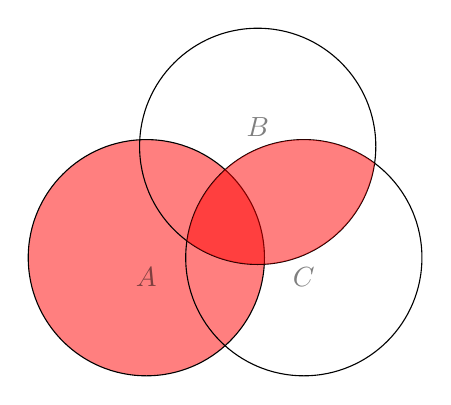
\begin{tikzpicture}
\begin{scope}[shift={(3cm,-5cm)}, fill opacity=0.5]
\fill[red] \firstcircle;

\draw \firstcircle node[below] {$A$};
\draw \secondcircle node [above] {$B$};
\draw \thirdcircle node [below] {$C$};

\clip \secondcircle;
\clip \thirdcircle;
\fill[red]\thirdcircle;
\end{scope}
\end{tikzpicture}

\subsubsection{Wahrscheinlichkeitsbegriff}
\begin{axiom}
	Jedem Ereignis $A$ aus dem Ereignisfeld $F$ ordnet man eine nichtnegative Zahl $P(A)$ zu. Das ist die \textit{Wahrscheinlichkeit}.
\end{axiom}
\begin{axiom}
	 $P(\Omega)=1$
\end{axiom}
\begin{axiom}
	Sind Ereignisse $A_i$; $i\in {1,..,n}$ paarweise unvereinbar, d.h: $A_i A_j = \emptyset$ mit $i \neq j $ so gilt $P(A_1+A_2+ \ldots A_n) = P(A_1+P(A_2)+\ldots+P(A_n) )$ Daraus ergeben sich folgende Eigenschaften für Wahrscheinlichkeiten:
	\begin{itemize}
		\item $P(\emptyset)= 0$
		\item $P(\bar{A}) = 1 - P(A)$, $\bar{A} = \Omega -A$
		\item $ 0 \leq P(A) \leq 1$
		\item Für $A \subset B$ (A ist Teilereignis von B) folgt $P(A) \leq P(B)$
		\item $P(A+B) = P(A)+P(B)-P(AB)$
		\item  $P(A_1 + A_2+ \ldots +A_n) \leq P(A_1) + P(A_2)+ \ldots+P(A_n)$
	\end{itemize} 	
\end{axiom}
 
%Vorlesung 2
\subsubsection{Bedingte Wahrscheinlichkeit}
Eine Wahrscheinlichkeit von A unter der Bedingung dass B eingetreten ist schreibt man als $P(A|B)$
\[P(A|B) = \frac{P(AB)}{P(B)}\]
Motivation: Gegeben seien $n$ unvereinbare, gleich wahrscheinliche Ereignisse \\
\begin{tabular}{ll}
  $A_1,A_2,...,A_n$ & mit $m$ günstig für A \\
 & mit $k$ günstig für B \\ 
 & mit $r$ günstig für AB (r $\leq$ k, r $\leq$ m) \\ 
\end{tabular}
\[ P(A|B)=\frac{r}{k}=\frac{\frac{r}{n}}{\frac{k}{n}}=\frac{P(AB)}{P(B)} \]

\begin{exmp}
	Zwei Würfel werden geworfen. Wie groß ist die Wahrscheinlichkeit die Summe 8 zu erhalten (A), falls bekannt ist, dass die Summe gerade ist(B)\\
	\[ P(A)=\frac{5}{36}, P(B)=\frac{1}{2}, P(AB)=\frac{5}{36} \]
	\[ P(A|B)=\frac{P(AB)}{P(B)}=\frac{5}{18} \]
\end{exmp}


\paragraph{Bayes'sche Formel} 
Seien $A_1,A_2,...,A_n$ unvereinbar 
\[ P(A_i|B)=\frac{P(B|A_i) P(A_i)}{\sum\limits_{j=1}^n P(B|A_j) P(A_j)} \]

\subsubsection{Diagnostische Verfahren - Anwendung von Wahrscheinlichkeit}
Es seien $D^+, D^-$ zwei mögliche Krankheitszustände (krank, gesund) und $T^+,T^-$ die zwei möglichen Ergebnisse eines diagnostischen Tests.
So bezeichnet man:
\begin{itemize}
 \item $P(D^+)$ : Prävalenz
 \item $P(T^+|D^+)$ : Sensitivität
 \item $P(T^-|D^-)$ : Spezifizität
 \item $P(D^+|T^+)$ : positiv-prädiktiver Wert (PPV)
 \item $P(D^-|T^-)$ : negativ-prädiktiver Wert (NPV)
\end{itemize}

\subsection{Zufallsvariablen und Verteilungsfunktionen}
Qualitative Beschreibung aus Gedenko: ``Eine \underline{Zufallsgröße}(-variable) ist eine Größe, deren Werte vom Zufall abhängen und für die eine Wahrscheinlichkeitsfunktion existiert''
Jedem Elementarereignis $\omega \in \Omega$ (unzerteilbar) wird eine reelle Zahl zugeordnet $X=X(\omega) : \Omega = \mathbb{R}$ und $F_x(t):=O(X<t)$ wird als Verteilungsfunktion der Zufallsgröße $X$ definiert. Sie ist monoton nicht fallend, linksseitig stetig und gehorcht den Bedingungen $F(-\infty)=0,F(\infty)=1$ \\
$\rightarrow$ Umkehrung: jede solcher Funktionen lässt sich als Verteilungsfunktion deuten

\subsection{Wichtige Vereilungsfunktionen}
\paragraph{Binomialverteilung}
\[ P_n(m)=\binom{n}{m}p^m q^{n-m} \] 
wobei \[ \binom{n}{m}:=\frac{n!}{m!(n-m)!}, q:= 1-p \] 

\[ F(x)=
  \begin{cases}
    0 & x \leq 0 \\
    \sum\limits_{k<x}P_k & 0 < x \leq n \\
    1 & x > n
  \end{cases}
\] 

\paragraph{Poissonverteilung}
\[ P_n=\frac{\lambda e^{\lambda}}{n!}, \lambda > 0 \]

\[ F_{\lambda}(t)=\sum_{k=0}^t \frac{\lambda^k}{k!}e^{-\lambda} \]

\paragraph{Normalverteilung}
\[ F(x)=\phi(x)=\frac{1}{\sigma\sqrt{2\pi}} \]

\[ \int_{-\infty}^x e^{\frac{-(z-a)^2}{2\sigma^2}} dz , \sigma > 0 \]

\subsection{Erwartungswert, Varianz, weitere Momente}
\textbf{Erwartungswert} $E(X)$ eine Zufallsgröße:\\
\underline{diskret} $E(X)=\sum_i x_i p_i$ wobei $x_i$: mögl. Werte, $p_i$: Wahrscheinlichkeiten \\

\begin{exmp}
	Würfel 
	\[ E(X)=\frac{1}{6} \sum_{i=1}^6 i = \frac{21}{6} = \frac{7}{2} \]
\end{exmp}
\begin{exmp}
	Binomialverteilung: 
	\[ E(X)= \sum_{k=0}^n k P_n(k) = \sum_{k=0}^n k \binom{n}{k} p^k(1-p)^{n-k} \] 
	Nebenrechnung:
	\[ k \binom{n}{k} = \frac{k n!}{k! (n-k)!} = \frac{n!}{(k-1)!(n-k)!} = \frac{n(n-1)!}{(k-1)!(n-k)!} = n \binom{n-1}{k-1} \] 
	\[\rightarrow E(X)= n \sum_{k=1}^{n} \binom{n-1}{k-1} p^k (1-p)^{n-k} = np \sum_{k=1}^n \binom{n-1}{k-1} p^{k-1} (1-p)^{n-k} \] 
	Sei $k'=k-1, n'=n-1$ \\
	\[ \rightarrow E(X)=np \underbrace{\sum_{k=0}^{n'} \binom{n'}{k'} p^{k'}(1-p)^{n'-k'}}_{=1} = np \]
	
	\underline{stetig} 
	\[ E(X)=\int x - p(x) dx , \quad p(x): \text{Wahrscheinlichkeitsdichte} \]
\end{exmp} 

\begin{exmp}
	Uniformverteilung auf Intervall $[a,b]$
	\[ E(X)= \frac{1}{b-a} \int_{a}^b x dx =  \frac{b^2 - a^2}{2(b-a)} = \frac{1}{2}(b+a) \]
\end{exmp}


\begin{exmp}
	Normalverteilung
\[ E(X)= \frac{1}{\sigma \sqrt{2 \pi}} \int_{-\infty}^{\infty} x e^{\frac{-(x-a)^2}{2\sigma^2}} dx \]
\[ x' = \frac{x-a}{\sigma} \rightarrow x = \sigma x' + a ,\quad dx= \sigma x' \]
\[ E(X) = \frac{\sigma}{\sigma \sqrt{2 \pi}} \int_{- \infty}^{\infty} (\sigma x' + a) e^{\frac{-x^2}{2}} dx' \]
ungerade Funktion ergibt 0
\[ E(X) = \frac{\sigma}{\sqrt{2 \pi}} \underbrace{\int_{- \infty}^{\infty} e^{-x' 2/2} dx'}_{=\sqrt{2 \pi}} = a \]
\end{exmp}

\textbf{Varianz} (oder Dispersion)
\[ V(X) := E \big[ (X-E(X)^2) \big] \]
\underline{diskret}: 
\[ V(X) = \sum\limits_{i} \big[ x_i - E(x) \big] ^2 * p_i \]
\underline{stetig}: 
\[ V(X) = \int \big[ x_i - E(x) \big] ^2 * p(x)\; dx \]


%Vorlesung 3
\[
V(X) := E[(EX)-X)^2] = E[E(X)^2 - 2X E(X) + X^2]  = E(X^2) - [E(X)]^2
\]
Bsp. Würfel
\[
V(X) = \dfrac{1}{3} \left[\left(\dfrac{5}{2}\right)^2 + \left(\dfrac{3}{2}\right)^2 + \left(\dfrac{1}{2}\right)^2\right] = \dfrac{35}{12}
\]
Bsp. Uniformverteilung [a,b]
\begin{align*}
V(X) &= \dfrac{1}{b-a} \int_a^b \! x^2 \, \mathrm{d}x - \left(\dfrac{b+a}{2}\right)^2\\
&= \dfrac{b^3 - a^3}{3 (b-a)} - \dfrac{(b+a)^2}{4} \\
&= \dfrac{(b-a) (b^2+a^2+ab}{3(b-a)} - \dfrac{(b+a)^2}{4}\\
&= \dfrac{1}{12} (4b^2+4a^2+4ab-3b^2-6 ab-3a^2)\\
&= \dfrac{1}{12} (b^2-a^2-2ab) \\
&= \dfrac{(b-a)^2}{12}
\end{align*}
\paragraph{Definition}
Wir bezeichnen $m_k$ als das \underline{gewöhnliche Moment} (oder Anfangsmoment)\\
k-ter Ordnung $m_k := E(X^k)$, \\
diskret also $\sum_i\left(x_i\right)^k p_i$,
stetig $\int \! x^k (p(x) \, \mathrm{d}x$
\\
Das \underline{zentrale Moment} (auf Zentrum Erwartungswert bezogen) k-ter Ordnung \\
$\mu_k := E\left[(X-m_1)^k\right]$. Die Varianz ist also das zweite Zentralmoment $V(X) = \mu_2 = m_2 - (m_1)^2$.\\
Man kann immer $\mu_k$ durch $m_l$ $\left( l \leq k\right)$ ausdrücken.

\subsection*{1.6 Korrelation}
\paragraph{} Eine Erweiterung dieser Momente stellt die \underline{Kovarianz}
$b(X,Y) := E\left[\left(X-E(X)\right) \left( Y-E(Y) \right)\right]$
dar (gemischte Zentralmomente zweiter Ordnung).

Es gilt offensichtlich $b(X,X) = V(X)$.\\
Die normierte Größe $\rho(X,Y) := \rho_{X,Y} = \dfrac{b(X,Y)}{\sqrt{V(X)V(Y)}}$ bezeichnet man als \underline{Korrelationskoeffizient}. \\
Es gilt: $-1 \leq \rho \leq 1$. Für $X=Y$ gilt $\rho = 1$ und für $X=-Y$ gilt $\rho = -1$. \\
Falls $X$ und $Y$ unabhängig dann gilt $\rho = 0$ (nicht aber umgekehrt).\\
Anwendung auf Wahrscheinlichkeiten: \\
$E(X) = p_X$, $V(X) = p_X(1 - p_X)$ \\

$\rho_{X,Y} = \dfrac{p_{XY} - p_Xp_Y}{\sqrt{p_X(1-p_X) p_Y(1-p_Y)}}$
$\rightarrow p_{XY} = p_Xp_Y + \rho_{X,Y} \sqrt{p_X(1-p_X)p_Y(1-pY)}$

\paragraph{Grenzfälle}
$\rho = 0$ : $p_{XY} = p_X p_Y$\\
$\rho = 1$\footnote{$\rightarrow p_X = p_Y$} : $p_{XY} = (p_X)^2 + p_X(1-p_X) = p_X$\\
$\rho = -1$\footnote{$\rightarrow p_X = 1 - p_Y$} : $p_{XY} = p_X(1-pX) - p_X(1-p_X) = 0 $\\

\subsection*{1.7 Einige wichtige Gesetze der Wahrscheinlichkeitstheorie}

\subsubsection*{Gesetz der großen Zahlen}
Bernoulli: Für alle $\epsilon > 0$: $\lim\limits_{n \rightarrow \infty}{P \left\lbrace| \dfrac{\mu}{n} - p | < \epsilon \right\rbrace} = 1$
\begin{itemize}
	\item $\mu$ - Anzahl der Ereignisse
	\item $n$ - Anzahl der Versuche
	\item $p$ - Wahrscheinlichkeiten der Ereignisse
\end{itemize}
%Vorlesung 4
Tschebyshew: Für ein $\epsilon >0$:
\[\lim\limits_{n \to \infty} P\{\frac{1}{n} \sum_{i=1}^{n} X_i - \frac{1}{n} \sum_{i=1}^{n} E(X_i)| < \epsilon \} = 1\] für eine Folge paarweise unabhängiger Zufallsgrößen.\\

$\{X_i\}_{i=1,2, \ldots n}$ mit gleichmäßiger beschränkter Varianz  $V(X_i) \leq C$


\subsubsection*{lokaler Grenzwertsatz von Mavre-Laplace}
Sei $0<p<1$ die Wahrscheinlichkeit eines Ereignisses.
In n-Versuchen gilt
\[P_n (m) = \binom{n}{m} p^m(1-p)^{n-m}\] So gilt \[\lim\limits_{n \to \infty} \frac{\sqrt{np(1-p)} P_n(m)}{\frac{1}{\sqrt{2 \pi}} e ^{-\frac{x^2}{2}}} \rightarrow  1 \text{ mit } x=\frac{m-np}{\sqrt{np(1-p)}}\]

\subsubsection*{zentraler Grenzwertsatz}

Sei $S_n =  \sum_{i=1}^{n} X_i$ mit $E(X_i)<\infty$, $V(X_i) = \sigma ^2 < \infty$

So gilt für jedes t
\[ \lim\limits_{n \rightarrow \infty} P(\frac{S_n - n E(X_i)}{\sqrt{n} \sigma}< t) = \frac{1}{\sqrt{2\pi} }\int_{-\infty}^{t} e^{\frac{-x^2}{2}} dx
\]

also: die Folge der Verteilungen der standardisierten Zufallsgröße konvergiert gegen die Standartnormalverteilung (d.h. a = 0, $\sigma$ = 1)


\section{Deskriptive Statistik}

\begin{itemize}
	\item Beschreibung von Daten und Kohorten ist zentral für das Verständnis einer Arbeit
	\item Ziel ist mit wenigen Kenngrößen das wesentliche zu charakterisieren 
	\item man gibt ''Punktschätzer''  für Erwartungswerte und ''Konfidenzintervalle'' (KI; engl. CI) als Maß für die Genauigkeit der Schätzung:\\
	$(1- \alpha) \text{ KI} [a,b] : P(a \leq \theta \leq b) = 1-\alpha$
\end{itemize}

\todo{Übersichtsbild Konfidenzintervall}

\subsection{Ein Merkmal}
\subsection{nominale und Ordinale Größen}
%nominal -- Kann man nur kategorisieren aber nicht ordnen
%ordinal -- kann man ist eine Kategoriale Größe die man in eine Reihenfolge bringen kann

\begin{itemize}
	\item absolute und relative Häufigkeiten (z.B Häufigkeitstabellen)
	\item grafisch: Balkendiagramme (mit Konfidenzintervall KI oder Standardfehler SE)
	\item Kreisdiagramm (verpönt)
\end{itemize}

\todo{Bespiel Balkendiagramm einfügen}
	
	$\hat{p} = \frac{r}{n}$ , $\hat{SE} = \frac{\hat{sd}}{\sqrt{n}}= \frac{\sqrt{\hat{V}}}{\sqrt{n}} = \sqrt{\frac{\hat{p} (1- \hat{p})}{n}}
KI \approx \hat{p} \pm 2 SE$, r= \#Fehlgeburten, n = \#Beobachtungen 


\subsubsection*{Metrische Daten}
\textbf{Lagemaß}
\begin{itemize}
	\item Mittelwert (arithmetisch oder geometrisch, d.h. log-Skala)
	\begin{itemize}
		\item übliche und ''robuste'' Methoden
		\item arithmetisch  = $\frac{1}{n}\sum_{i=1}^{n} X_i$
		\item geometrisch  = $[ \prod_{i=1}^{n} X_i]^{1/n}$
	\end{itemize}
-Median und andere Qunatile (verschiedene Schätzverfahren)
\end{itemize}
\textbf{Streumaß}
\begin{itemize}
	\item Standardabweichung (''sample'' - Methode) $sd^2 = \frac{1}{n-1} \sum_{i=1}^{n}(x_i - \bar{x})^2$
	\item Interquartilabstand (engl. interquartile range (IQR) z.B. 25. und 75. Perzentil)
	\item Spannweite
	\item grafisch: Histogramm, Boxplot	
\end{itemize}
\todo{Grafik Boxplot einfügen}

\subsection{Zusammenhang 2er Merkmale}
Nominal
\begin{itemize}
	\item Kontigenztafel: odds ration, relatives Risiko
	\item grafisch: forest plots
\end{itemize}
metrisch
\begin{itemize}
	\item Korrelationskoeffizient (mit KI)
	\item Streudiagramm
\end{itemize}

\subsection{Simpsons Paradoxon}
Grundidee: Effekt in Gesamtgruppe muss nicht ''echt'' sein. Er kann in Subgruppen anders ausfallen.

\begin{tabular}{|c|c|c|}
	\hline 
	& A & B \\ 
	\hline 
	Erfolg & 70 (30\%) &  50(22\%) \\ 
	\hline 
	Misserfolg & 160 & 182 \\ 
	\hline 
	Summe & 230 & 232 \\ 
	\hline 
\end{tabular} 

\begin{tabular}{|c|c|c|c|}
	\hline 
	&   & A & B \\ 
	\hline 
	Männer & E & 7 (20\%) & 45(21\%) \\ 
	\hline 
	& M & 28 & 175 \\ 
	\hline 
	Frauen & E & 63(32\%) & 5(33\%) \\ 
	\hline 
	& M  & 132 & 10 \\ 
	\hline 
\end{tabular} 

%Vorlesung 5
\section{Statistisches Testen}
\subsection{Die Logik des Testes}
Die Analogie zum Beweis durch Widerspruch kann hilfreich sein, hier ein Beispiel:\\
\begin{tabularx}{\linewidth}{|L|L|}  
\hline
Statistisches Testen & Beweis durch Widerspruch \\ \hline
-Annahme: $H_0: \mu_1 = \mu_2$ (Mittelwert d. Gruppe 1 ist MW d. Gruppe 2)  & -Annahme: $\sqrt{2}$ ist rational \\
-man glaubt nicht an Annahme & -man glaubt nicht an Annahme \\
-Folge: Wenn Ann. stimmt... & -Folge: Wenn Ann. stimmt... \\
-Kommt etwas sehr Unwahrscheinliches raus, so ist die Annahme nicht plausibel(Konvention $< 5\%$ dann wird $H_0$ abgelehnt) & -Kommt man auf einen Widerspruch, so muß die Annahme falsch sein \\
-Kommt etwas Plausibles raus, so weiß man wenig über die Annahme (KI kann helfen) & -Kommt man nicht auf einen Widerspruch, so weiß man evtl. wenig über die Annahme \\ \hline
\end{tabularx}
\begin{tabularx}{\linewidth}{|L|L|L|}
\hline
 & $H_0$ stimmt & $H_0$ stimmt nicht \\ \hline
 $H_0$ abgelehnt & Typ I Fehler \newline $\alpha$ \newline (Konvention $\alpha = 0.05$) & :) \newline Power: $1-\beta$ \\
 $H_0$ nicht abgelehnt & :) & Typ II Fehler\newline $\beta$ \newline Planung: $\beta=0.1 ... 0.2$ erstrebt... Sicherheit über $\beta$ hat man nicht \\ \hline
\end{tabularx}

\subsection{Der T-Test}
Vergleich zweier MW, $H_0: \mu_1 = \mu_2$ \\
Wir schätzen die ``t-Statistik'' (Annahme gleicher Varianz) \\
\[ T = \frac{\bar{x_1} - \bar{x_2}}{s \sqrt{\frac{1}{n_1} + \frac{1}{n_2}}} \]
\[ s^2 = \frac{(n_1 - 1) s_1^2 + (n_2 -1) s_2^2}{n_1 + n_2 -2} \]
n: Stichpunktgröße der i-ten Gruppe \\
$\bar{x_i}$: MW \\
$s_i^2 = \sum\limits_{j=1}^{n_i} (x_j^{(i)} - \bar{x}^{(i)} )^2 $ \\
($T = \frac{\Delta}{SE}$ ist die grundlegende Struktur) \\
Unter $H_0$: T hat ``t-Verteilung'' mit f-Freiheitsgraden
\[ f= n_1 + n_2 -2 \]
Welch-Test (keine Annahme zur Varianz) \\
\[ T = \frac{\bar{x}_1 - \bar{x}_2 }{\sqrt{\frac{s_1^2}{n_1} + \frac{s_2^2}{n_1}}} \]
t-Verteilung mit f Freiheitsgraden
\[ f=\frac{(\tilde{s_1}^2 + \tilde{s_2}^2)^2)}{\frac{\tilde{s_1}^4}{n_1 - 1} + \frac{\tilde{s_1}^4}{n_1 - 1}} \]
\[ \tilde{s_i} = \frac{s_i}{\sqrt{n_i}} \]
KI für $\Delta \mu$: $\Delta \bar{x} \pm \underbrace{t_{\alpha / 2 , f}}_{\sim 2 \text{ für } \alpha=0.05 \text{ und } f >> 1}  \cdot$ SE \\
p-Wert: Wahrscheinlichkeit den Wert von T zu beobachten unter $H_0$ \\
Ist der p-Wert $p_0$, so beinhaltet ein $(1-p_0)$-KI gerade so den Wert Null \\
z.B. Ist $p_0=0.05 \rightarrow$ das 95\%-KI erreicht die Null gerade so

\subsection{Kontingenztafel: $\chi^2$- und Fischer-Test}
Gegeben sei:
\begin{tabular}{c|c|c|c}
 & A & B \\ \hline
 I & $n_{11}$ & $n_{12}$ & $n_{1\cdot}$ \\ \hline
 II & $n_{21}$ & $n_{22}$ & $n_{2\cdot}$ \\ \hline
  & $n_{\cdot1}$ & $n_{\cdot2}$ & $n_{\cdot\cdot}$
\end{tabular}
\newline
$\frac{n_{11}}{n_{21}}$ schätzt das ``Odds'' (die Chance) von I im Vergleich zu II bei gruppe A. $\widehat{OR}=\frac{\frac{n_{11}}{n_{21}}}{\frac{n_{12}}{n_{22}}}$ schätzt das ``Odds Ratio'' (Chancenverhältnis) KI: $OR \cdot e^{\pm z_{a/2 \cdot SE}}$ \\
Hier ist die Frage, ob 1 im Intervall liegt (Null auf der log-Skala)\\
 Fisher-Test $\Leftrightarrow$ KI von OR (mit anderer Schätzmethode allerdings)  \\
Fischer-Test heißt ``exakt'', da ein strenger Wert aus der Kombinatorik berechnet wird
\[ p = \frac{\binom{n_{1\cdot}}{n_{11}} \binom{n_{2\cdot}}{n_{22}}}{ \binom{n_{\cdot \cdot}}{n_{\cdot1}}} \]
\[ \binom{n_{\cdot\cdot}}{n_{\cdot1}} = \frac{n_{12} + n_{22} + n_{12} + n_{21} }{n_{12} + n_{21} } \]

%Vorlesung 6
Der Zusammenhang nominaler Merkmale kann mit höherer Power mit dem (asymptotischen) $\chi^2$-Test als mit einem exakten Test überprüft werden.
\[ \chi^2 = \sum\limits_{i,j} \frac{(n_{ij} - e_{ij})^2}{e_{ij}} \]
\[ e_{ij}= \frac{n_{i\cdot} \times n_{\cdot j}}{n_{\cdot \cdot}} \]
$e_{ij}:$ erwartete Anzahl \\
$\chi^2$ hat $\chi^2$-Verteilung mit $f=(l-1)\cdot(k-1)$ Freiheitsgrade \todo{l= Anzahl an Zeilen, k= Anzahl Spalten der Kontigenztafel}\\
Faustregel: $n_{ij} \neq 0$ für alle $i,j$ und $< 20 \%$ der Zellen haben $l_{ij} < 5 \rightarrow \chi^2$-Test \\
%Ende der Vorlesung
\end{document}
